% !TXS template
\documentclass[french]{article}
\usepackage[T1]{fontenc}
\usepackage[utf8]{inputenc}
\usepackage{lmodern}
\usepackage[a4paper]{geometry}
\usepackage{babel}
\usepackage{hyperref}
\usepackage{amsmath}
\usepackage{amssymb}
\usepackage{commath}


\numberwithin{equation}{section}

\usepackage{graphicx}
\graphicspath{ {./images/} }

\title{Fonction Gamma $\Gamma$, Distribution Bêta $\beta$, Distribution de Dirichlet, Processus de Dirichlet}
\author{BONIN Alexandre}

\begin{document}

\maketitle

\tableofcontents

\section{Fonction Gamma $\Gamma$}

\subsection{Définition}

La fonction Gamma est une extension à l'ensemble des complexes $\mathbb{C}$ de la fonction factorielle définie sur les entiers. C'est à dire une fonction telle que :

\begin{equation}
\Gamma (n+1) = n! \quad (n \in \mathbb{N})
\end{equation}

\textit{On notera en particulier qu'on obtient la factorielle de $n - 1$, et non pas de n.}
\\

Et définie pour tout complexe par :

\begin{equation}
\Gamma (z) = \int_{0}^{+\infty} t^{z-1} e^{-t} \dif t \quad (z \in \mathbb{C})
\end{equation}

Cette fonction respecte la propriété suivante des factorielles pour les complexes :

$$\Gamma(z+1) = z \Gamma(z)$$

\begin{figure}[h]
	\centering
	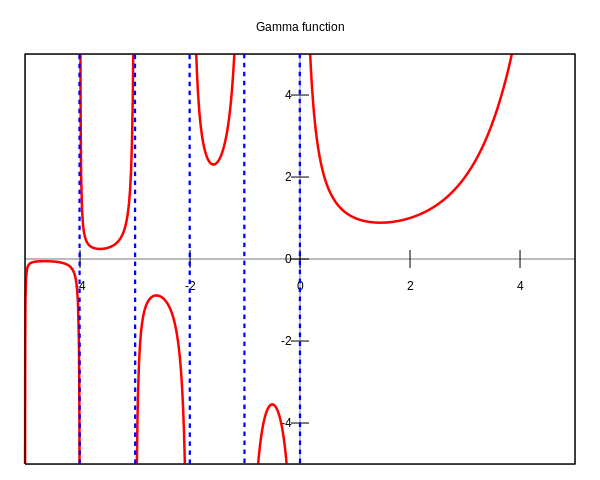
\includegraphics[width=0.5\textwidth]{600px-Gamma_plot.svg}
	\caption{Plot de la fonction gamma sur $\mathbb{R}$}
\end{figure}

\begin{figure}[h]
	\centering
	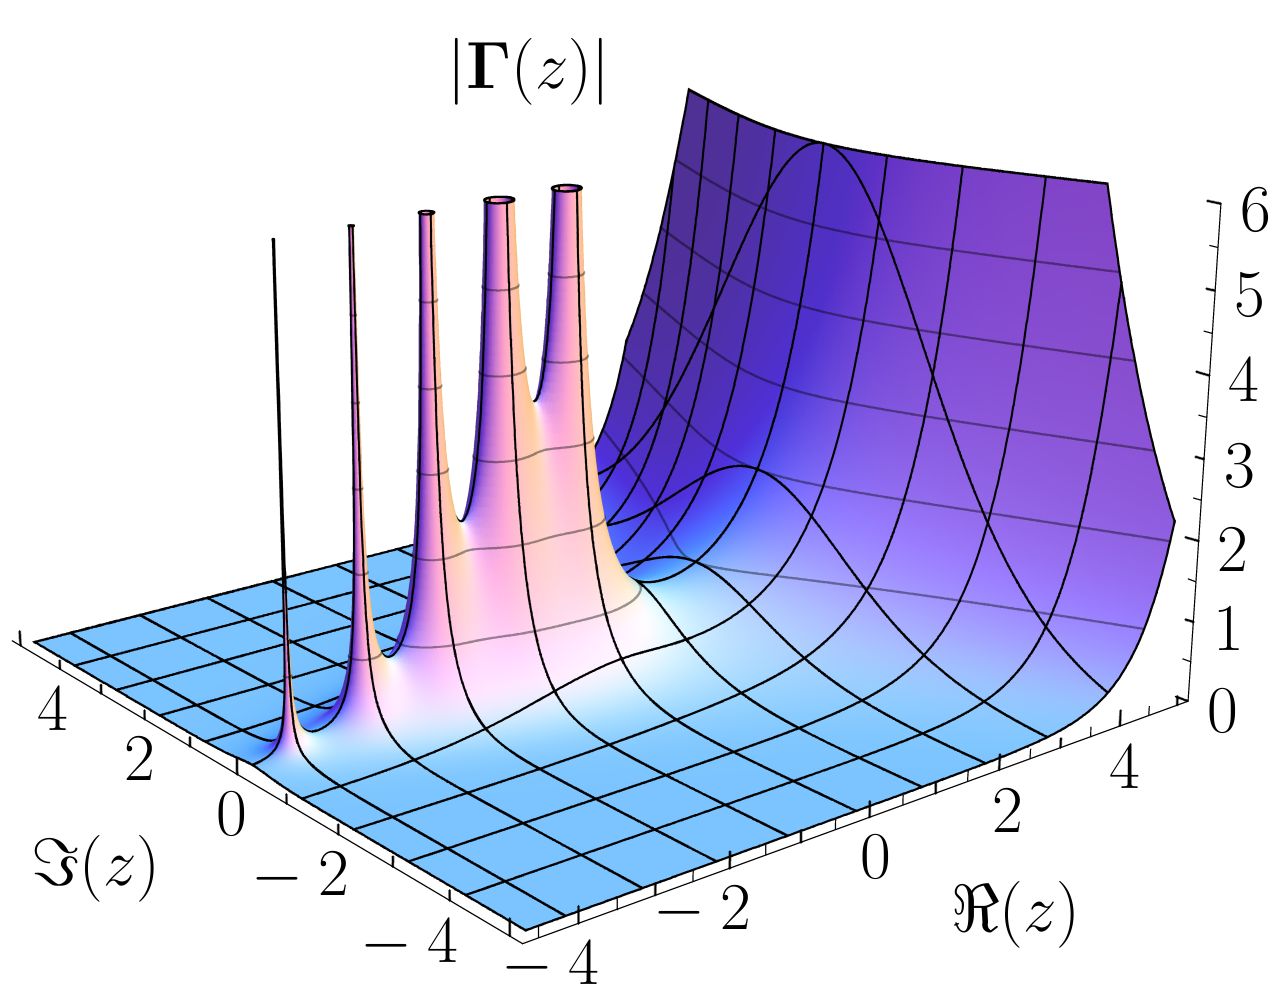
\includegraphics[width=0.5\textwidth]{Gamma_abs_3D}
	\caption{Plot de la fonction gamma sur $\mathbb{C}$}
\end{figure}


\subsection{Calculs utiles}

\subsubsection{Dérivée}

La dérivée p-ième de $\Gamma$ est donnée sur $\mathbb{R}_+^*$ pour un $p \in \mathbb{N}$ par:

\begin{equation}
\Gamma^{(p)}(x) = \int_{0}^{+\infty} (\ln t)^p t^{x - 1} e^{-t} \dif t
\end{equation}

\textit{La fonction $\Gamma$ est infiniment dérivable sur $\mathbb{R}_+^*$}

\subsubsection{Logarithme}

L'équation fonctionnelle du logarithme de $\Gamma$ est la suivante:

\begin{equation}
\ln \Gamma(z) = \ln \Gamma(z + 1) - \ln(z)
\end{equation}

Dont on peut tirer l'approximation suivante pour un grand réel $z$:

\begin{equation}
\ln \Gamma(z) \approx (z - \frac{1}{2}) \ln z - z + \frac{1}{2} \ln(2\pi)
\end{equation}

Et pour un petit réel $z$ :

\begin{equation}
\ln \Gamma(z - m) = \ln \Gamma(z) - \sum_{k=1}^{m} \ln (z - k)
\end{equation}

\subsubsection{Fonction digamma}

La dérivée logarithmique de la fonction $\Gamma$ est appelée fonction \textit{digamma} et est utilisée dans certain calculs comme pour la dérivée de la fonction Bêta. La fonction digamma est définie par :

\begin{equation}
\label{digamma}
\text{digamma}(z) = \frac{\partial}{\partial z} \ln \Gamma(z) = \frac{\Gamma'(z)}{\Gamma(z)}
\end{equation}

\section{Distribution Bêta}

\subsection{Définition}

La distribution $\beta$ est une loi définie sur [0, 1]. Elle est paramétrée par deux réels (souvent appelés \textit{shape parameters}) $\alpha$ et $\beta$.

On note qu'une V.A. X suit une loi Bêta par :
\[
X \sim Beta(\alpha, \beta) 
\]

Et la fonction de densité est définie par :

\begin{equation}
f(x; \alpha, \beta) = \frac{x^{\alpha - 1} (1 - x)^{\beta - 1}}{B(\alpha, \beta)}
\end{equation}

Où la fonction $\beta$ est une fonction liée à gamma :

\begin{equation}
\text{B}(\alpha, \beta) = \frac{\Gamma(\alpha)\Gamma(\beta)}{\Gamma(\alpha + \beta)}
\end{equation}

Où définie en ses propres termes par :

\begin{equation}
\text{B}(\alpha, \beta) = \int_{0}^{+\infty} \frac{t^{x-1}}{(1+t)^{x+y}}\dif t
\end{equation}

\begin{figure}[h]
	\centering
	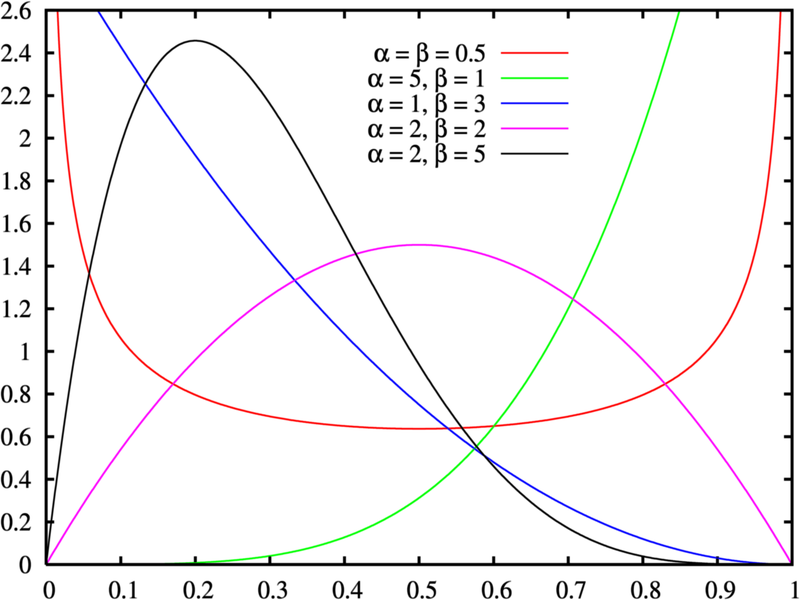
\includegraphics[width=0.5\textwidth]{Beta_distribution_pdf}
	\caption{Densité de probabilité de Bêta}
\end{figure}

\begin{figure}[h]
	\centering
	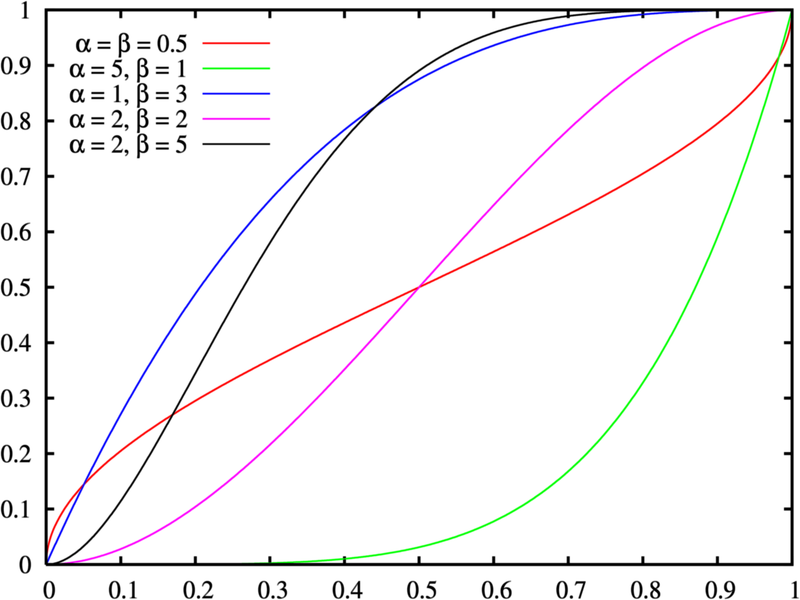
\includegraphics[width=0.5\textwidth]{800px-Beta_distribution_cdf}
	\caption{Fonction de répartition de Bêta}
\end{figure}

\subsection{Moments}

\subsubsection{Moyenne}

\[ X \sim Beta(\alpha, \beta) \]
\begin{equation}
\mathbb{E}[X] = \frac{\alpha}{\alpha + \beta}
\end{equation}

\subsubsection{Mode}

\begin{equation}
\arg\max p(x) = \frac{\alpha - 1}{\alpha + \beta - 2} \quad \text{pour} \quad \alpha, \beta > 1
\end{equation}

\subsubsection{Variance}

\begin{equation}
\text{Var}[X] = \frac{\alpha \beta}{(\alpha + \beta)^2(\alpha + \beta + 1)}
\end{equation}

\subsection{Propriétés de la fonction Bêta}

La fonction Bêta est symétrique :

\[
\text{B}(x, y) = \text{B}(y, x)
\]

Si x et y sont deux entiers strictement positifs, alors la fonction est définie par un coefficient binomial:

\begin{equation}
x, y \in \mathbb{N^*} \implies \text{B}(x, y) = \binom{x+y}{x}
\end{equation}

\subsection{Calculs utiles}

\subsubsection{Dérivée}

\begin{equation}
\frac{\partial}{\partial x} \text{B}(x, y) = \text{B}(x, y) \left( \frac{\Gamma'(x)}{\Gamma(x)} - \frac{\Gamma'(x+y)}{\Gamma(x+y)} \right) = \text{B}(x, y)( \psi(x) - \psi(x+y))
\end{equation}

Où $\psi$ représente la fonction digamma (\ref{digamma}).

\section{Distribution de Dirichlet}

\subsection{Définition}

La distribution de Dirichlet est une généralisation à plusieurs dimensions de la loi Bêta. On parle de loi pour des V.A. multinomiales (des multinômes, donc plusieurs V.A.). La loi de Dirichlet n'est pas paramétrée par deux réels $(\alpha, \beta)$ comme la loi Bêta mais par un vecteur de $K$ paramètres réels positifs non nuls (de $]0, +\infty]$) $(\alpha_1, ..., \alpha_K)$ qui permettra de générer un K-nome $(x_1, ..., x_K)$. \\

On note qu'une V.A. multinomiale X suit la loi de Dirichlet paramétrée par le vecteur $\alpha$ par :

\[ X \sim Dir(\alpha) \]

La fonction de densité du K-nome est définie par :

\begin{equation}
f(x_1, ..., x_K; \alpha_1, ..., \alpha_K) = \frac{1}{\text{B}(\alpha)} \prod_{i=1}^{K}x_i^{\alpha_i - 1}
\end{equation}

Où B est la fonction Bêta multinomiale (soit la fonction Bêta de la distribution Bêta, pour un nombre $K$ de paramètres). La forme suit celle de sa version à $K=2$ :

\[ \text{Soit} \quad \alpha = (\alpha_1, ..., \alpha_K) \]

\begin{align}
\text{B}(\alpha) \quad &= \quad \frac{\Gamma(\alpha_1) * ... * \Gamma(\alpha_K)}{\Gamma(\alpha_1 + ... + \alpha_K)} \nonumber\\
&= \quad \frac{\prod_{k=1}^{K} \Gamma(\alpha_k)}{\Gamma(\sum_{k=1}^{K} \alpha_k)}
\end{align}

Des restrictions sont posées sur les variables:

\begin{itemize}
	\item $x_i > 0$ pour tout $i$
	\item $\sum_{j=1}^{K} x_j = 1$
\end{itemize}

\bigskip

L'ensemble des points qu'il est possible de générer par cette loi est donc un simplexe de dimension K - 1 puisque la V.A. $x_K$ est déduite par 
\[ x_K = 1 - \sum_{j=1}^{K} x_j\]
On a donc $K - 1$ degrés de liberté. Le simplexe est de plus ouvert car 
\[ \forall j \in [1, K], \quad \sum_j x_j = 1 \land x_j > 0 \implies x_j < 1 \]
Ainsi les points de la frontière du simplexe sont exclus.

\section{Processus stochastique}

\subsection{Définition}

Un processus stochastique est généralement une suite (temporelle ou simplement indexée sans notion de temps) de variables aléatoires. Plus généralement on peut indexer les variables par n'importe quel ensemble, ainsi on formalise la notion comme telle:\\

Soit un certain espace probabilisé $(\Omega, \cal{F}, P)$ où $\Omega$ est l'univers, $\cal{F}$ une tribu (aka $\sigma$-algèbre) de $\Omega$ qui représente l'ensemble des événements, et $P$ une mesure de probabilité. Soit X un processus stochastique, X est défini comme :

\[ 
X = \left\{ X(t, \omega); t \in T, \omega \in \Omega \right\}
\]
où $T$ est l'ensemble d'indexation. $X$ est valué sur un certain espace mesurable $(S, \Sigma)$.\\

X est donc une fonction à deux variables, l'indexation $t$ et l'élément $\omega$ de l'univers.

\begin{enumerate}
	\item Si on fixe $t$, on obtient alors une variable aléatoire $X_t(\omega)$ sur $\Omega$ valuée dans $S$.
	\item Si on fixe $\omega$, on obtient alors l'évolution "temporelle" (Ou simplement l'évolution selon t) de $X(\omega)$ : 
	\[ (X(t, \omega))_{t \in T} \]
	on appelle cette valeur la trajectoire du processus stochastique. Dans le cas de valeurs de T plus générales que des entiers naturels, on la note sous forme fonctionnelle :
	\[ \omega \in \Omega, \quad t \mapsto X(t, \omega) \]
	ou de façon identique
	\[ t \mapsto X_t(\omega) \]
\end{enumerate}
\bigskip



\section{Processus de Dirichlet}

\subsection{Définition}

Un processus de Dirichlet est un processus stochastique dont la réalisation est une distribution sur un certain espace probabilisable $(\Theta, \Sigma)$ où $\Theta$ est l'univers et $\Sigma$ une tribu.\\

Soit $A = \left\{ A_i \right\}_{i=1, ..., K}$ un partitionnement de $\Theta$ mesurable ($A_k \in \Sigma$). Soit G la réalisation du processus de Dirichlet, alors le processus de Dirichlet est défini par :

\begin{equation}
(G(A_1), ..., G(A_K)) \sim Dir(\alpha H(A_1), ..., \alpha H(A_K))
\end{equation}
où $H$ représente la distribution "moyenne" du processus, et $\alpha$ est le paramètre de concentration (à quel point on s'éloigne ou colle à la moyenne $H$). \\

$H(A_i)$ donne la probabilité moyenne pour la partition $A_i$. Cette probabilité initiale est systématiquement multipliée par le paramètre de concentration $\alpha$. On obtient ainsi $\alpha H(A_i) = d_i$, tel que la distribution de Dirichlet utilisée devient :

\[ Dir(d_1, ..., d_K) \]
\textit{C'est à dire une distribution de Dirichlet paramétrée par un certain vecteur réel positif $d$}\\

La distribution $Dir(\alpha H(A_1), ..., \alpha H(A_K))$ donne un vecteur aléatoire $(x_1, ..., x_K)$, et ainsi $x_i = G(A_i)$, soit la mesure de probabilité généré aléatoirement pour la partition $A_i$, par le processus de Dirichlet. On obtient bien ainsi une mesure de probabilité aléatoire sur $A$, i.e. une distribution aléatoire.\\

Voir le processus du "restaurant chinois" pour un exemple visuel et intuitif d'une réalisation du processus de Dirichlet : \url{https://topicmodels.west.uni-koblenz.de/ckling/tmt/crp.html?parameters=0.5&dp=1}. Plusieurs réalisations du processus du restaurant résultera en un nombre différents de tables, avec des probabilités différentes pour chacune d'elle. L'histogramme ainsi obtenu nous montre à chaque réalisation une forme différente, soit une distribution différente.\\

Le processus de Dirichlet est vu comme une généralisation infini-dimensionnelle de la distribution de Dirichlet en cela qu'elle permet de générer potentiellement une infinité de table (on peut partitionner $\Theta$ en un $A$ arbitrairement grand), là où la distribution de Dirichlet produit un vecteur de taille $K$ fixé d'avance. On peut donc dire que la distribution de Dirichlet est un cas particulier du processus de Dirichlet avec un partitionnement fixé tel que $\left|A\right| = K \in \mathbb{N}$.

\end{document}
